\subsubsection{Tuned comparison - Optimized settings \label{tunedComparison}}
In this section we will conduct experiments comparing the optimized Cross Entropy against the
optimized CMA obtained from the sections, \ref{GamesPerAgentCE} and \ref{OptimalSettingsCMA}.
The chosen optimal settings for each of the algorithms is specified in the following tables
\begin{table}[h]
\centering
\begin{tabular}{l r}
Optimizer & CMA\\
Number of Evaluations & 40000\\
Number of Learning Games & 30\\
Population size& 50\\
Parent size & 25\\
Games per Agent & 5\\
Tetris Type & Normal\\
\hline
Recombination Type & LINEAR\\
Initial Sigma & 0.5\\
 & \\
\end{tabular}
\quad
\begin{tabular}{l r}
Optimizer & Cross Entropy\\
Number of Evaluations & 40000\\
Number of Learning Games & 30\\
Population size & 200\\
Parent size & 50\\
Games per Agent & 1\\
Tetris Type & Normal\\
\hline
Sigma & 100\\
Noise Type & Constant\\
Noise & 4
\end{tabular}
\caption{Optimized Cross Entropy and CMA for comparison experiments}
\end{table}

\textbf{Results}\\

\begin{figure}[H]
	\centering
	\captionsetup[subfigure]{justification=centering}
    \begin{subfigure}[b]{0.49\textwidth}
    	\caption{Cross Entropy}
        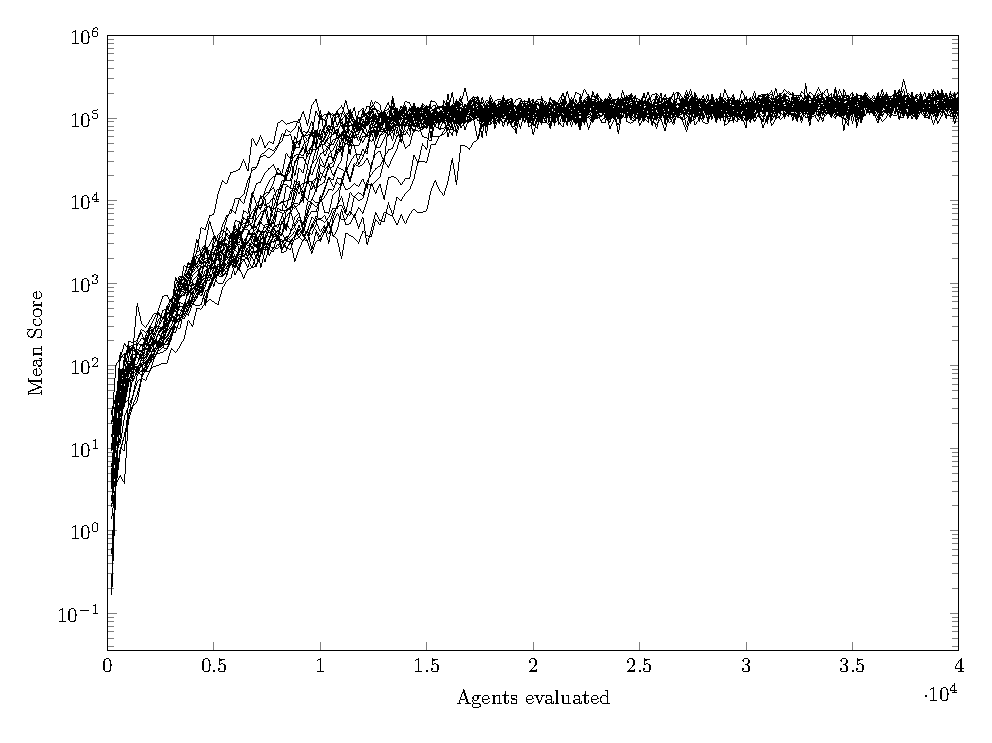
\includegraphics[width=\textwidth]{data/TunedComparison/CE_Optimal_Bertsekas_NormalTetris/PlotFile.pdf}
    \end{subfigure} 
    \begin{subfigure}[b]{0.49\textwidth}
    	\caption{CMA}
        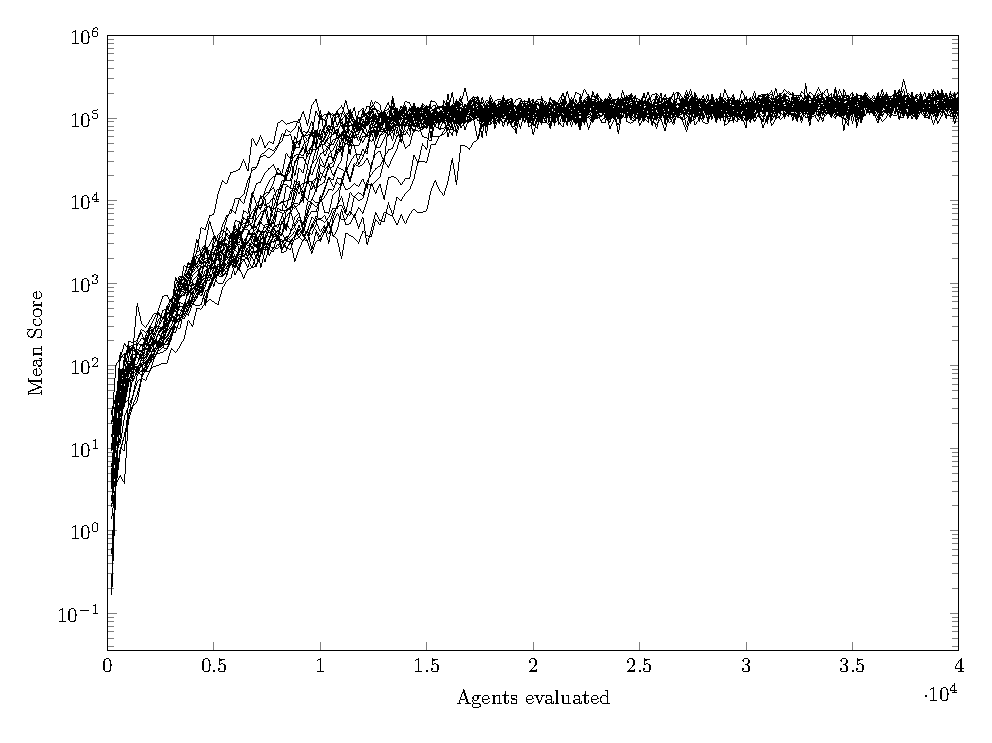
\includegraphics[width=\textwidth]{data/TunedComparison/CE_Optimal_Bertsekas_NormalTetris/PlotFile.pdf}
    \end{subfigure}

    \caption{30 experiment with optimal settings Cross Entropy and CMA}
\end{figure}

\begin{figure}[H]
\centering
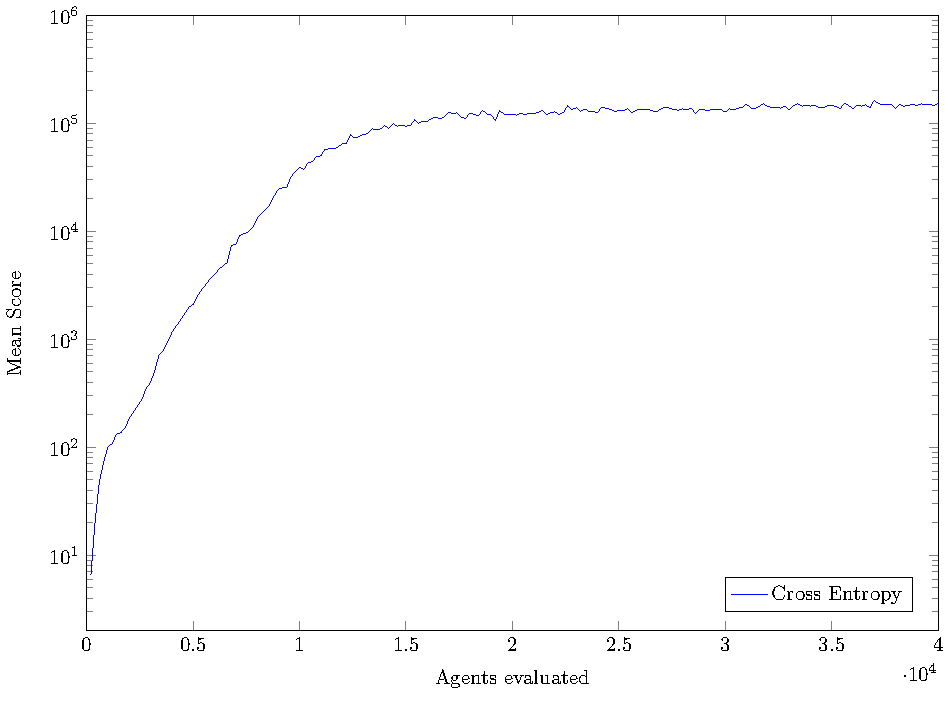
\includegraphics[scale=1]{data/TunedComparison/mean_CE_CMA/PlotFile.pdf}
\caption{Mean plot of optimal settings Cross entropy and CMA}
\end{figure}


\textbf{Analysis and discussion}\\

